%!TEX root = ../../thesis.tex
\chapter[Bounce-averaged drifts]{Bounce-averaged drifts}
\label{chap: BAD}
\begin{figure}
    \centering
    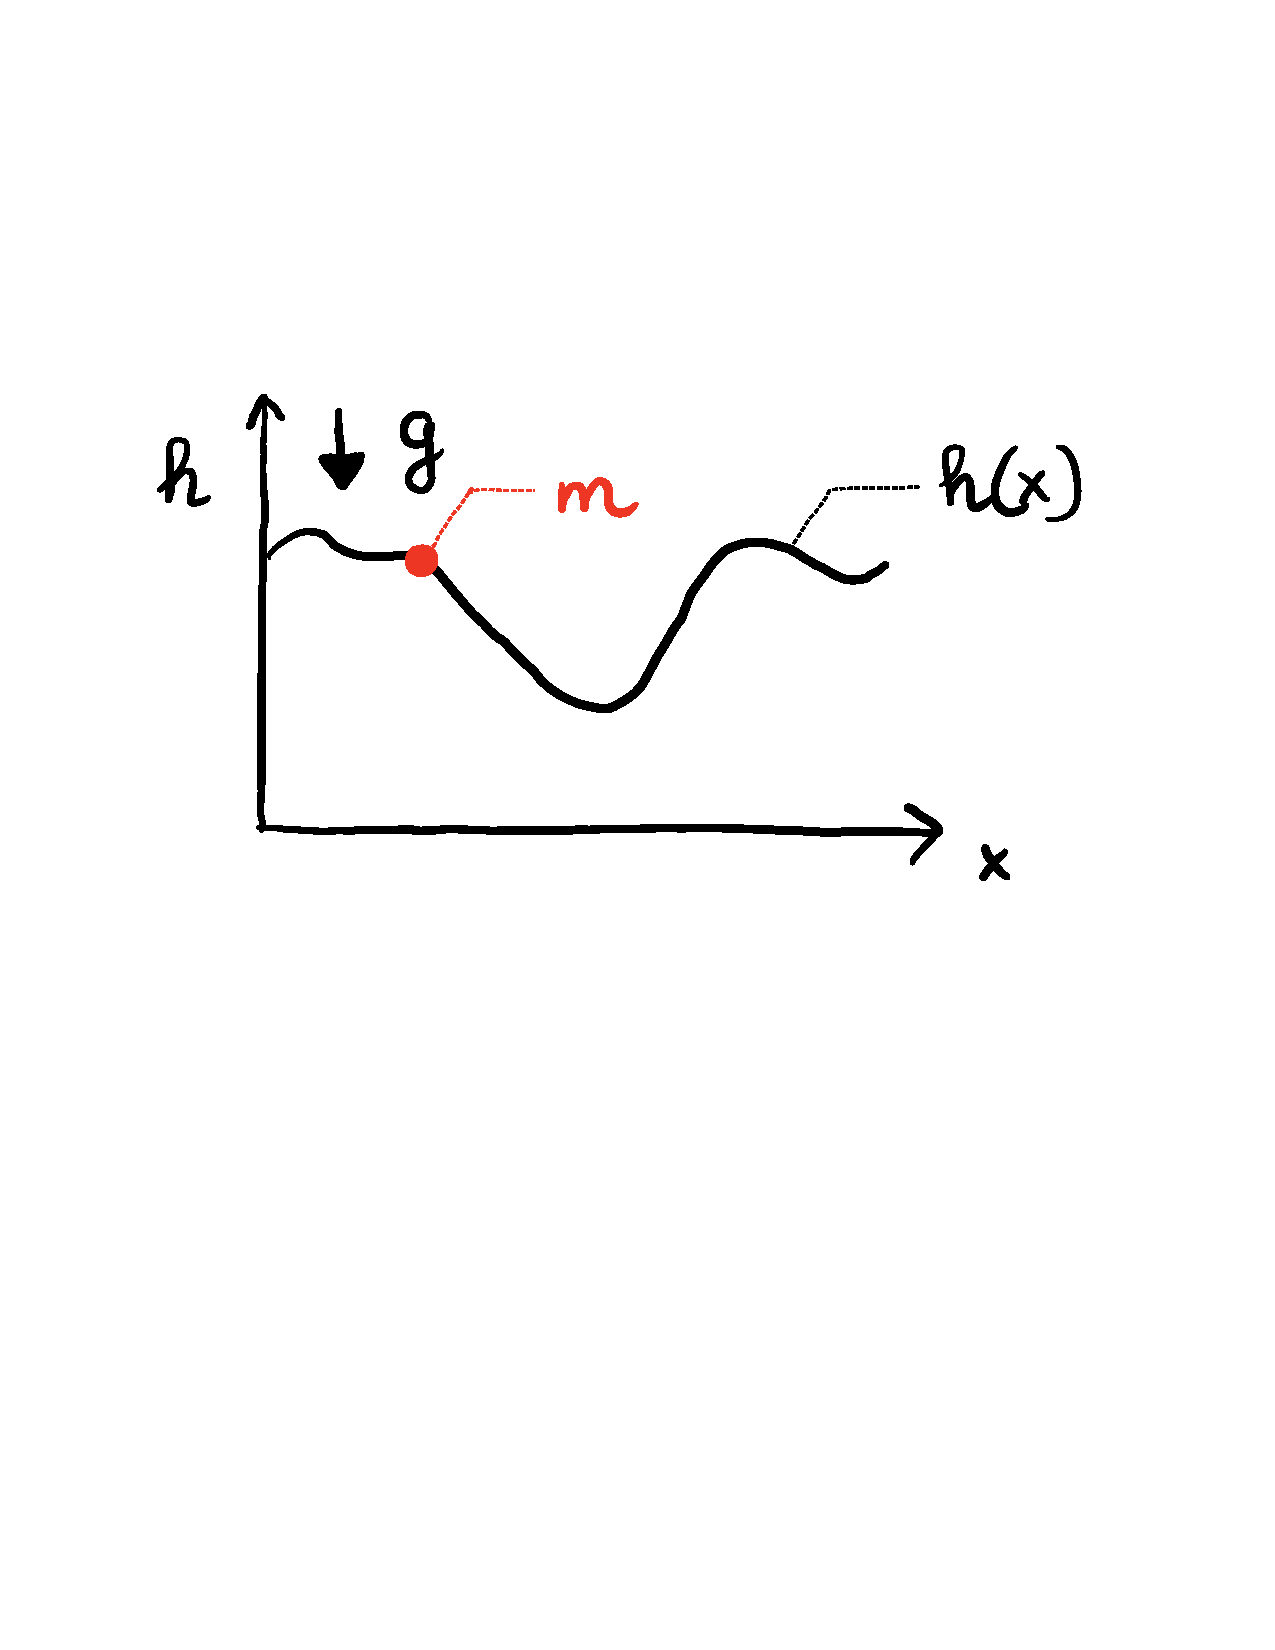
\includegraphics[width=0.5\textwidth]{3_chapters/1_papers/BAD/figures/bead-on-a-wire.pdf}
    \caption{A bead of mass $m$ in red, on a stiff wire prescribed by $h(x)$ in black, in a gravitational field with acceleration $g$.}
    \label{fig:bead on a wire}
\end{figure}
In the calculation of the \AE{} of trapped electrons, one requires accurate methods to calculate the bounce averaged drift a trapped particle experiences. Such a bounce-average is the time-average of some quantity which a trapped particle experiences, which may be thought of analogously to a bead on a stiff wire. This may be seen as follows: the total energy may be written as
\begin{equation}
    E = \mu B + \frac{1}{2}mv_\parallel^2 \implies v_\parallel = \pm \sqrt{\frac{2}{m}} \sqrt{E - \mu B}.
\end{equation}
Let us compare this quantity against the total energy of a bead on a wire in a gravitational field of constant acceleration, of which a sketch is given in Fig. \ref{fig:bead on a wire}. Here the total energy is given by
\begin{equation}
    E = mg h(x) + \frac{1}{2}mv^2 \implies v = \pm \sqrt{\frac{2}{m}} \sqrt{E - mgh(x)}.
\end{equation}
The equivalence is now obvious: the perpendicular energy $\mu B$ may be interpreted as a potential $mgh$. The bounce average of any quantity for the bead on a wire, which we denote by means of angular brackets, may now simply be thought of as
\begin{equation}
    \langle \dots \rangle \equiv \frac{ \int_{\rm bounce} \dots \mathrm{d} t }{ \int_{\rm bounce} \mathrm{d} t } = \frac{ \int_{\rm bounce} \dots \frac{\mathrm{d} \ell}{\sqrt{E - mgh}} }{ \int_{\rm bounce} \frac{\mathrm{d} \ell}{\sqrt{E - mgh}} },
    \label{eq: bounce average analogy}
\end{equation}
where the region of integration is one periodic motion of the point mass on the wire, and we have used the fact that $v = \mathrm{d}\ell/\mathrm{d}t$ with $\mathrm{d}\ell$ being the distance travelled by the point mass $m$ in time $\mathrm{d} t$. \par 
Though constructed by means of an analogy, Eq. \eqref{eq: bounce average analogy} may be used to readily find various properties emblematic of bounce-averages. Firstly, regions where the point mass is reflected (which will be referred to as bounce-points) have $v=0$, and the integrand becomes singular. Resolving this singular behaviour accurately is not a trivial task, and in the proceeding publication we put much emphasis on executing such integrals correctly numerically by including benchmark cases. Furthermore, if the bounce point approaches a local maximum, the point mass will spent all of its time near the local maximum and the time-average hence only cares about values near the local maximum. Again, if not this property is not handled properly, one may find erroneous bounce averages. By focusing on resolving such bounce-averaging integrals correctly the computational cost and accuracy of such calculations is greatly improved, which in turn will aid in the \AE{} calculations. Let us note in passing that this exercise in numerical rigour has found use outside of the current thesis as well, currently being used in works of P. Costello and E. Rodr\'iguez. Without further ado, the publication shall now be presented in unaltered shape.
\vfill \newpage

